\documentclass{beamer}

\input{../ts-glærur}
\usepackage{tikz}
\usetikzlibrary{automata,positioning}

\title{FOR3R - Stöðuvélar}

\begin{document}
\begin{frame}
\titlepage
\end{frame}

\section{Stöðuvélar}

\begin{frame}{Stöðuvélar}
\begin{itemize}
 \item Forrit fela oft í sér innbyggt ástand
 \item Hægt er að tákna ástandsbreytingar formlega með \emph{stöðuvélum}
 \item Skoðum sérstaklega ``forrit'' sem samþykkja eða hafna strengjum eftir ákveðnum mynstrum
\end{itemize}
\end{frame}

\begin{frame}{Að hafna eða samþykkja}
\begin{itemize}
 \item Sjáum fyrir okkur forritunarvandamál: ``Greinum á milli löglegra og ólöglegra strengja. Strengir sem eingöngu innihalda stafinn $a$ eru löglegir, aðrir eru ekki löglegir.''
 \begin{itemize}
  \item Strengurinn $aaaaa$ er löglegur
  \item Strengurinn $aaaba$ er ekki löglegur
 \end{itemize}
 \item Til að búa til stöðuvél fyrir þetta vandamál þurfum við:
 \begin{itemize}
  \item Leið til að tákna ástönd í forritinu
  \item Leið til að tákna færslu á milli ástandanna
  \item Leið til að tákna hvaða ástönd eru lögleg og hver ekki
 \end{itemize}
\end{itemize}
\end{frame}

\begin{frame}[fragile]{Lausn á fyrsta forritunarvandamálinu}
Getum leyst vandamálið (það að samþykkja strengi sem innihalda einungis stafinn $a$) með eftirfarandi aðferð:

\begin{verbatim}
Ástand = "í lagi"
Lesum strenginn inn, einn staf í einu
  Ef "í lagi" og stafur=a, þá "í lagi"
  Ef "í lagi" og stafur!=a, þá "ekki í lagi"
  Ef "ekki í lagi" og stafur=a, þá "ekki í lagi"
  Ef "ekki í lagi" og stafur!=a, þá "ekki í lagi"
\end{verbatim}
Getum táknað þessa aðferð myndrænt!
\end{frame}

\begin{frame}{Strengir sem innihalda bara a}
Gerum ráð fyrir að allt stafrófið séð $\sigma = \{a, b\}$. Táknum ``í lagi'' með tvöföldum hring, ``ekki í lagi'' með einföldum, og færslur á milli með merktum örvum. Þá má lýsa ``forritinu'' með:
\begin{center}
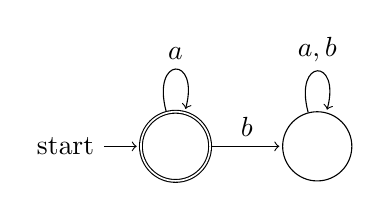
\begin{tikzpicture}[shorten >=1pt,node distance=1.8cm,on grid,auto] 
  \node[state,initial,accepting](q0) {$ $};
  \node[state] (q1) [right = of q0] {$ $};

  \path[->]
  (q0) edge node {$b$}(q1)
  (q0) edge [loop above] node {$a$} ()
  (q1) edge [loop above] node {$a,b$} ()
	;
\end{tikzpicture}
\end{center}
\end{frame}

\begin{frame}{Hvaða strengi samþykkir þessi stöðuvél?}
\begin{center}
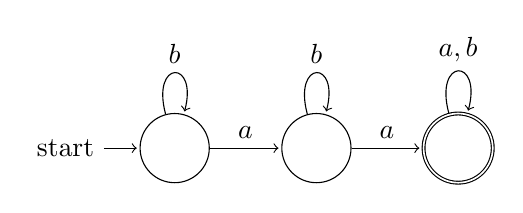
\begin{tikzpicture}[shorten >=1pt,node distance=1.8cm,on grid,auto] 
  \node[state,initial](q0) {$ $};
  \node[state] (q1) [right = of q0] {$ $};
  \node[state,accepting] (q2) [right = of q1]	{$ $};

  \path[->]
  (q0) edge [loop above] node {$b$} ()
  (q0) edge node {$a$}(q1)
  (q1) edge [loop above] node {$b$} ()
  (q1) edge node {$a$}(q2)
  (q2) edge [loop above] node {$a, b$} ()
	;
\end{tikzpicture}
\end{center}
\pause
Þá strengi sem byrja á stöfunum $aa$.
\end{frame}

\begin{frame}{Fleiri vandamál}
\begin{itemize}
 \item Strengir sem samanstanda af $ab$ endurtekið
 \item Strengir sem innihalda stafinn $a$
 \item Strengir sem enda á stafnum $a$
\end{itemize}
\end{frame}

\section{Reglulegar segðir}

\begin{frame}{Reglulegar segðir}
\begin{itemize}
 \item Reglulegar segðir eru notaðar til að tákna mynstur af þessu tagi á knappan máta:
 \begin{itemize}
 \item Strengir sem samanstanda af $ab$ endurtekið: $(ab)^*$
 \item Strengir sem innihalda stafinn $a$: $b^*ab^*$
 \item Strengir sem enda á stafnum $a$: $b^*a$
\end{itemize}
 \item Staðhæfing: Allar reglulegar segðir má tákna með þessari gerð af stöðuvél, og allar stöðuvélar af þessari gerð má setja fram með reglulegri segð
\end{itemize}
\end{frame}

\section{Öflugri stöðuvélar}

\begin{frame}{Öflugri stöðuvélar}
\begin{itemize}
 \item Þessi gerð af stöðuvélum (deterministic finite automata) dugar til að samþykkja og hafna strengjum sem hægt er að setja fram með einföldum reglulegum segðum
 \item Til þess að framkvæma almenna útreikninga þarf öflugri stöðuvélar
 \item Sé ótakmörkuðu minni bætt við stöðuvélina erum við komin með stöðuvél sem líkist svokallaðri \emph{Turing vél}
 \begin{itemize}
  \item Staðhæfing: Turing-vél getur lýst öllum útreikningum sem alvöru nútímatölva getur framkvæmt
 \end{itemize}
\end{itemize}
\end{frame}


\end{document}
